\documentclass[11pt]{beamer}

\usetheme{Rochester}
\definecolor{UBCblue}{rgb}{0.04706, 0.13725, 0.26667} % UBC Blue (primary)
\usecolortheme[named=UBCblue]{structure}

\usepackage[utf8]{inputenc}

\usepackage[english]{babel}

\usepackage{amsmath}
\usepackage{amsfonts}
\usepackage{amssymb}
\usepackage{graphicx}
\DeclareMathOperator {\argmin}{argmin}

\author{\small Jakob Pirs (XX-XXX-XX, jakob.pirs@uzh.ch)\\
Nina Erminia Cantoni (17-709-221, ninaerminia.cantoni@uzh.ch)\\
Rohit Koonireddy (XX-XXX-XX, rohit.koonireddy@bf.uzh.ch)\\
Yunxiang Guo (XX-XXX-XX, yunxiang.guo@uzh.ch)\\}

\title{Cryptocurrencies and the risk-free rate}


\setbeamertemplate{navigation symbols}{} 

\institute[]{University of Zurich, Department of Banking and Finance} 
\date{\today} 


% ---------------------------------------------------------

\bibliographystyle{apalike} %not used

%\bibliographystyle{abbrv}
%\setbeamertemplate{bibliography item}{\insertbiblabel}

% ---------------------------------------------------------

\begin{document}

\begin{frame}
\titlepage
\end{frame}

% ---------------------------------------------------------

\begin{frame}{Research Question}
 \centering Is there a relationship between cryptocurrencies and the 10 year treasury rate?
\end{frame}

\begin{frame}{Overview}
\tableofcontents 
\end{frame}

% ---------------------------------------------------------

\section{Data}
\begin{frame}{Data}
Through an API we accessed price data from yahoo over a period of 5 years (2018-2022). Finally, the data set comprises:
 \begin{itemize}
        \item 4 crytpocurrencies: \\
        Bitcoin 
\includegraphics[width=0.05\textwidth]{images/Bitcoin.png}, Ethereum 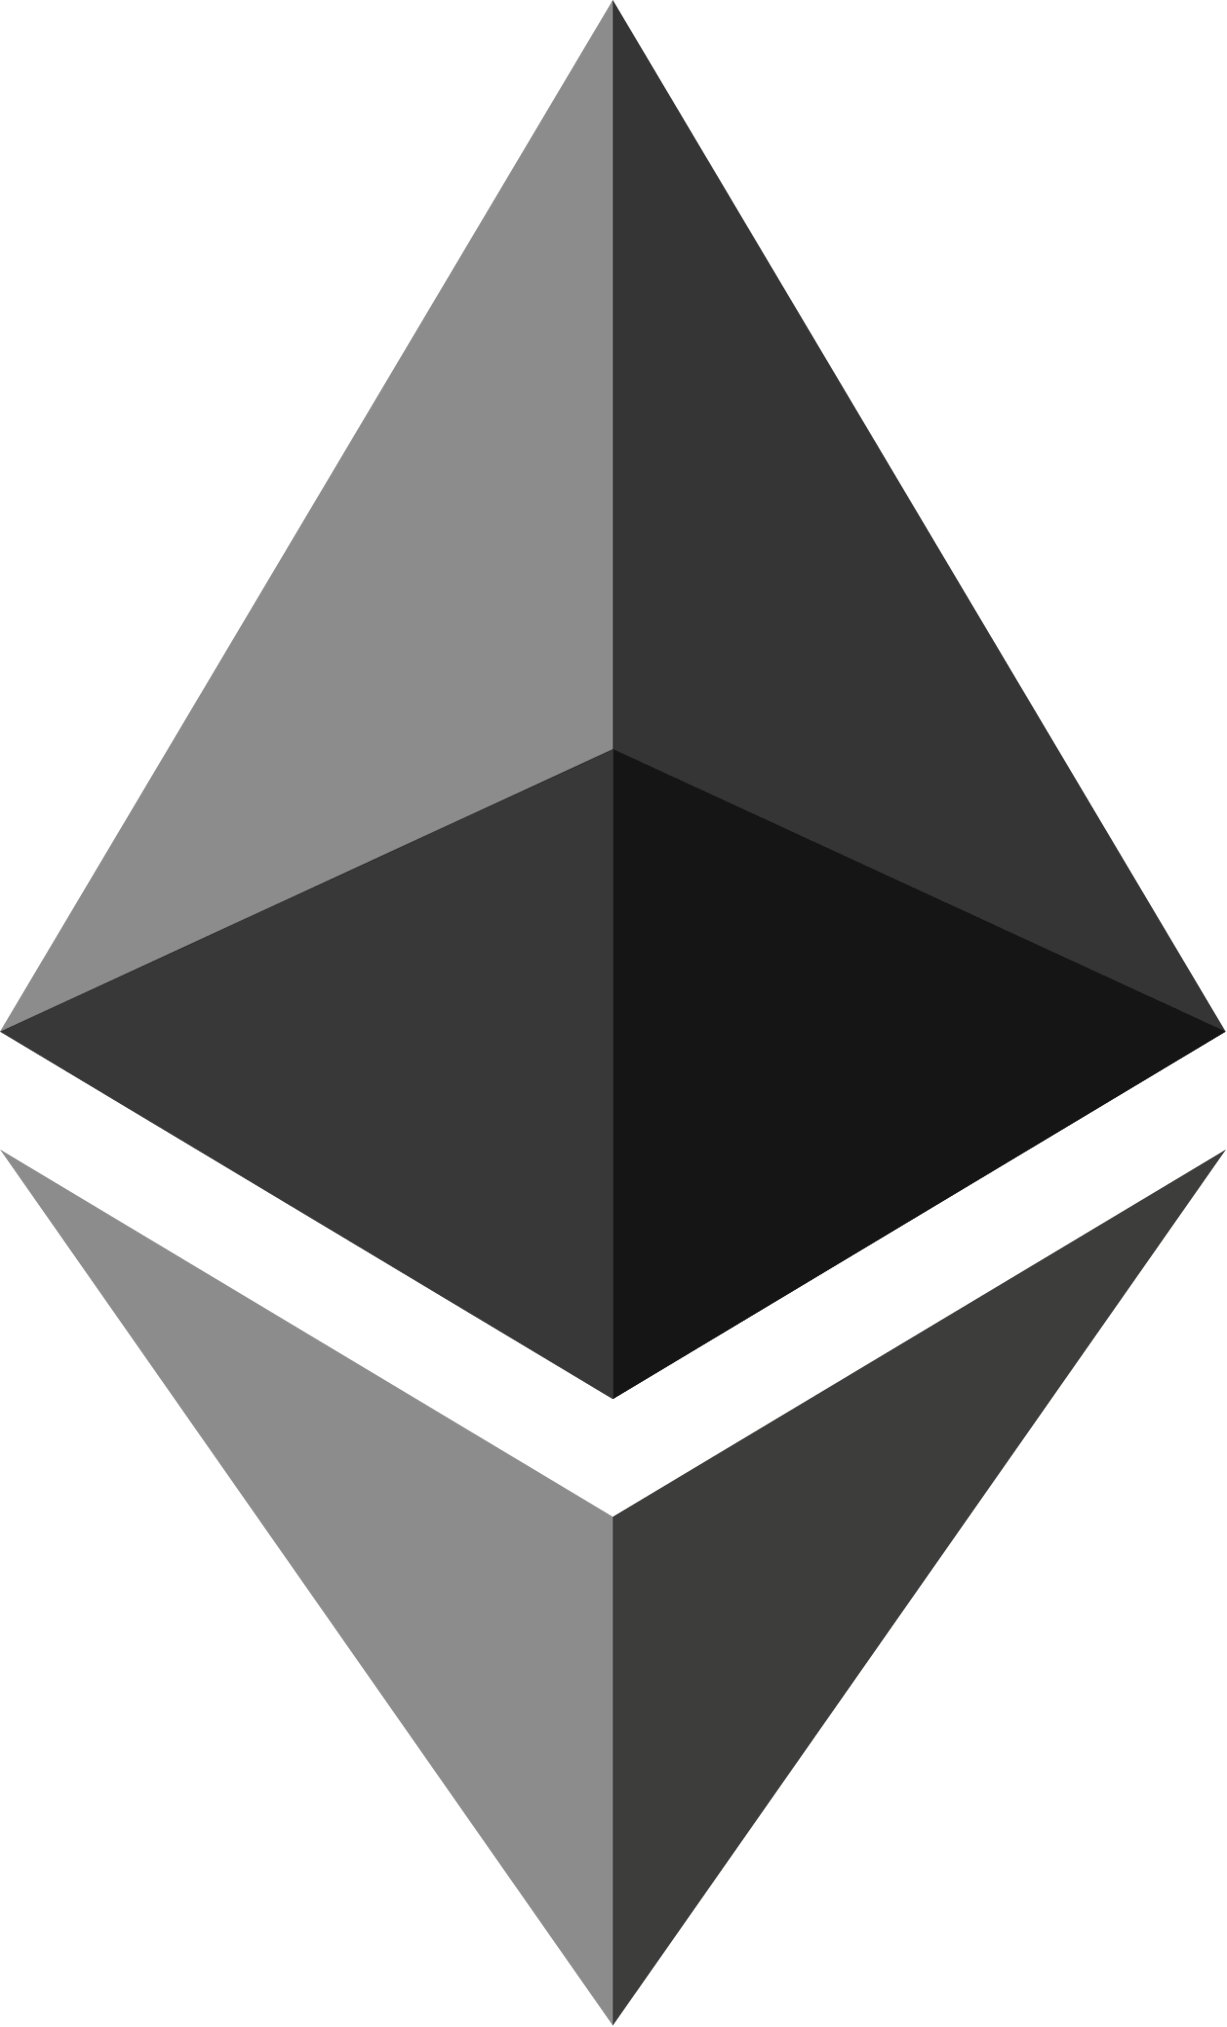
\includegraphics[width=0.035\textwidth]{images/ETH.png}, XRP 
\includegraphics[width=0.05\textwidth]{images/XRP.png}, Litecoin 
\includegraphics[width=0.05\textwidth]{images/LTC.png}
        
        \medskip
        
        \item CMC Crypto 200 Index
        
        \medskip
        
        \item 10 Year US Treasury Rate
    \end{itemize}

\end{frame}

% ---------------------------------------------------------

\begin{frame}{Data}
  \centering
    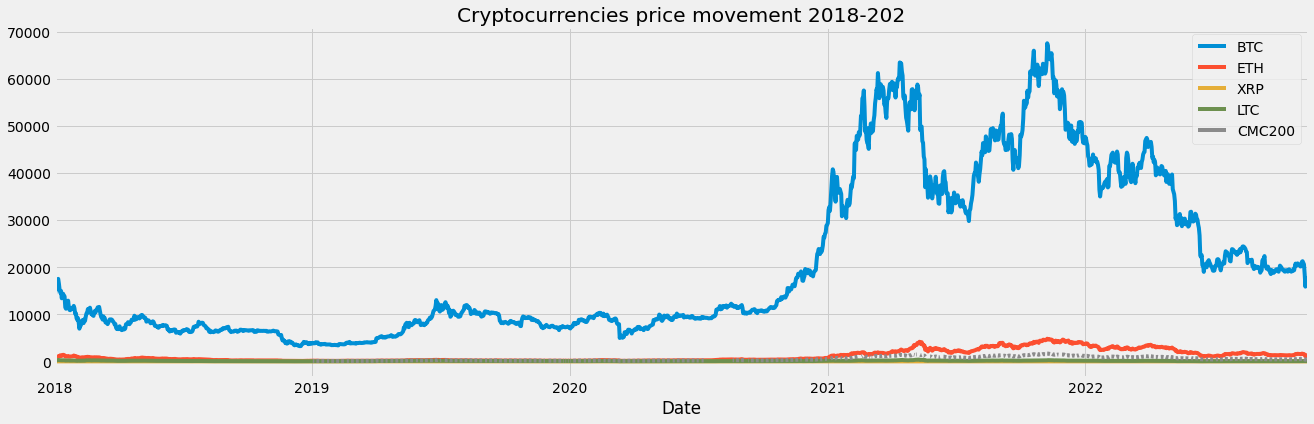
\includegraphics[width=9cm,keepaspectratio]{images/movement_crypto.png}
    
    \vspace{2}
    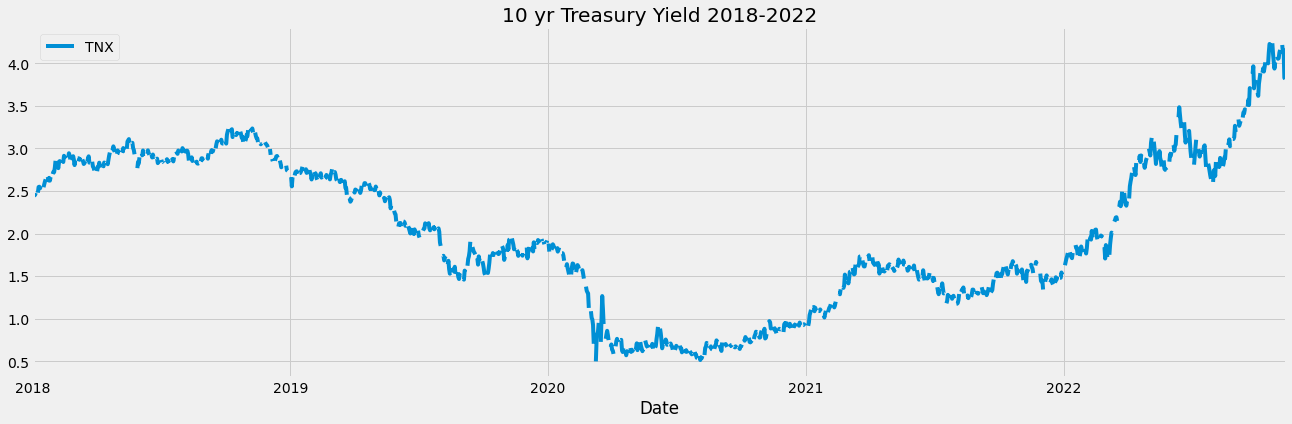
\includegraphics[width=9cm,keepaspectratio]{images/movement_treasury.png}\\
     
\tiny{\textit{Note.} Own representation.}
\end{frame}

% ---------------------------------------------------------

\section{Methodology}
\begin{frame}{Methodology}
We measure the relationship through:
    
    \begin{enumerate}
        \item Covariance
        \item Pearson's Correlation (linear)
        \item Spearman's Correlation (monotonic)
    \end{enumerate}
\end{frame}

% ---------------------------------------------------------
\section{Results}
\begin{frame}{Results - 1. Covariance}

    \centering
    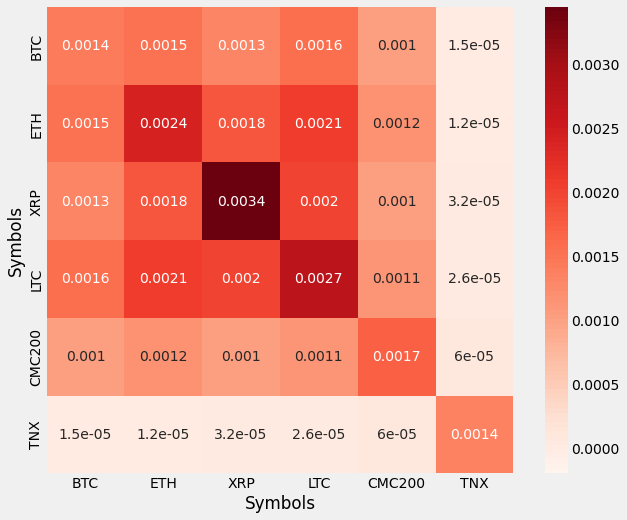
\includegraphics[height=7cm,keepaspectratio]{images/covariance_heatmap.png} \\

\tiny{\textit{Note.} Own representation.}
\end{frame}

% ---------------------------------------------------------


\begin{frame}{Results - 2. Pearson’s Correlation (linear)}

    \centering
    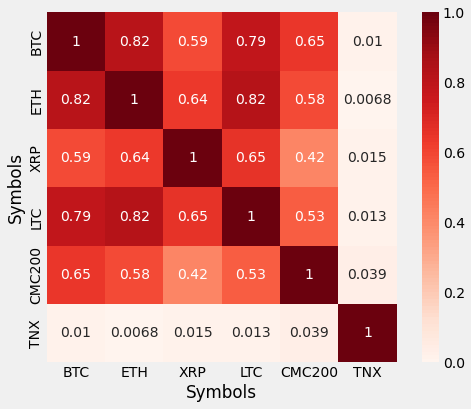
\includegraphics[height=7cm,keepaspectratio]{images/pearson_heatmap.png}

\tiny{\textit{Note.} Own representation.}
\end{frame}

% ---------------------------------------------------------

\begin{frame}{Results - 3. Spearman’s Correlation (monotonic)}
\centering
    (The Spearman's correlation did not give further insights.)
\end{frame}

% ---------------------------------------------------------

\section{Conclusion}
\begin{frame}{Conclusion}
    \begin{itemize}
    \item Close-to-zero covariance
    \item Negligible correlation ($<$0.1)
    \end{itemize}
    
\vspace{20}
    
\fbox{\parbox{\linewidth}{\textbf{No significant correlation between hikes in the risk-free rate and cryptocurrency returns.}}}
\end{frame}

% ---------------------------------------------------------

\begin{frame}

\begin{center}
    Thank you!


    \vfill
    \tiny{This presentation is part of the final project for Digital Tools for Finance (L) (03SMDFOEC008) by Igor Pozdeev, Department of Banking and Finance, University of Zurich. Refer to GitHub for the full project.}
\end{center}

\end{frame}

\end{document}